\begin{figure}
\centering
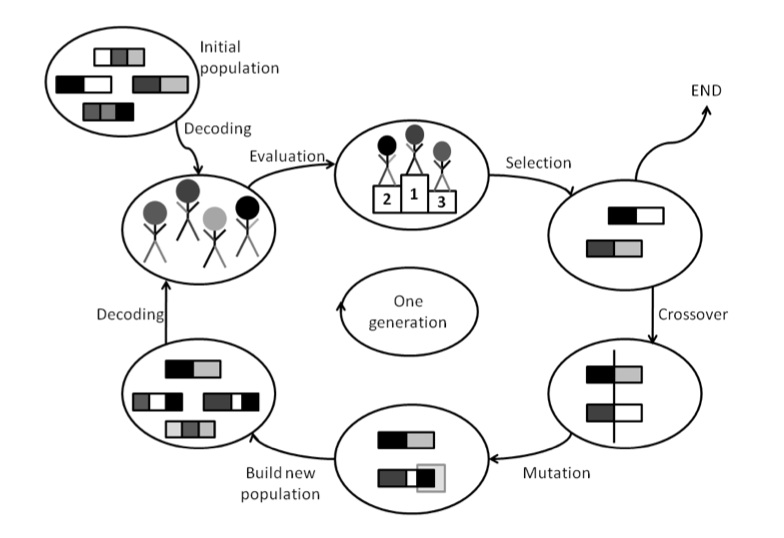
\includegraphics[width=0.5\textwidth]{img/working_principle_of_EA.jpg}
\caption{Evolutionary algorithms traditionally operate in a generation-based loop that, over the course of many iterations, gradually refines a population of candidate solutions, which is initialized with randomly-generated individuals, to generate increasingly fit individuals. That is, individuals that provide an increasingly satisfactory solution to a particular problem. At the start of each cycle of the loop, individual solutions are generated from a population of genotypes. These solutions are scored by a fitness function, which measures the performance of the individual as a solution to the problem. Then, the genetic material of fit individuals are mutated and recombined to create the next generation of candidate individuals. Once a predefined stopping criterion is met, usually a maximum number of generations or threshold fitness score, the evolutionary cycle is halted \cite{Prothmann2009EvolutionaryOptimisation}}.
\label{fig:working_principle}
\end{figure}